\subsection{Use cases}


I opgaven er spillet, udarbejdet ud fra en række Use cases. Use cases beskriver det spillet skal bruges til at en bruger/spiller. 

\begin{itemize}
    \item Spil spil
    \item Kast terning
    \item Vælg farve/brik
    \item Køb felt
    \item Brug chancekort
    \item Betal husleje
\end{itemize}

De ovenstående use cases er illustreret i Figur \ref{fig:ucDiagram}

\begin{figure}[!h]
    \centering
    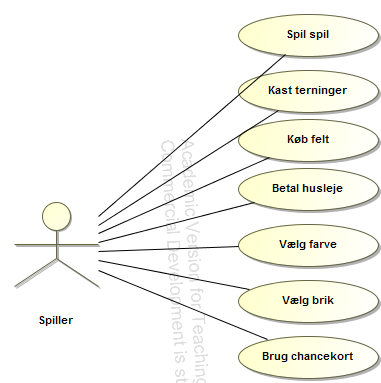
\includegraphics[]{sources/5_analyse/diagram.PNG}
    \caption{Use case diagram}
    \label{fig:ucDiagram}
\end{figure}


\newpage
Herunder i tabel \ref{table:uc1} er use casen Spil spil blevet beskrevet fully dressed

\begin{center}
\begin{longtable}{ |l|p{10.7cm}|} 
 \hline
 Use case  & Spil spil \\ 
 \hline
 Omfang & UC1 \\ 
 \hline
 Mål & Spilleren påbegynder spillet, for et antal spillere. \\ 
 \hline
  Primær aktør & Spilleren \\ 
 \hline
  Interessenter & De andre medspillere \\ 
 \hline
  Startbetingelser  & Spilleren vil gerne spille spillet \\ 
 \hline
  Succes kriterie & Spillet starter med det valgte antal spillere \\ 
 \hline
  Hoved succes Scenarie & 
  
  \begin{minipage}[t]{1\textwidth}
  \begin{enumerate}
      \item 2-4 personer vil gerne spille spillet.
      \item Spillet startes op på computeren
      \item Der vælges et antal spillere fra 2-4
      \item Der vælges navn for spillerne
      \begin{itemize}
          \item Spiller 2-4 vælger navn 
          \newline
          \emph{gentag indtil alle spiller har valgt navn}.
      \end{itemize}
      \item Der vælges farve for spillerne
      \begin{itemize}
          \item Spiller 2-4 vælger farve 
          \newline
          \emph{gentag indtil alle spiller har valgt en farve}.
      \end{itemize}
      \item Der vælges en brik til alle spillerne
      \begin{itemize}
          \item Spiller 2-4 vælger brik 
          \newline
          \emph{gentag indtil alle spiller har valgt en brik}.
      \end{itemize}
      \item Spillet starter med de valgte navne, farver og brikker.
  \end{enumerate} 
  \end{minipage}
  \\
 \hline
 Udvidelser & 
\begin{minipage}[t]{1\textwidth}
 \begin{itemize}
     \item Der indtaster mindre eller flere spillere end 2-4
        \begin{enumerate}
            \item Spillet giver en fejlbesked
            \item Spilleren ændrer antal spillere
            \item forsætter fra 3. i hoveddelen
        \end{enumerate}
    \item Der indtastet en forkert farve for en af spillerne
    \begin{enumerate}
        \item Spillet giver en fejlbesked
        \item Spillet lukker ned
    \end{enumerate}
    \item Der vælges en forkert brik, eller en brik der er optaget
    \begin{enumerate}
        \item Spillet giver en fejlbesked
        \item Spilleren vælger en anden brik
        \item fortsætter fra 7. i hoveddelen
    \end{enumerate}
 \end{itemize}
\end{minipage}
 
 \\
 \hline
 Specielle krav & Ingen \\
 \hline
 Teknologi- og dataformats-variationer & Ingen \\
 \hline
 Hyppighed & Hver gang spillet starter fra ny \\
 \hline
 Diverse & Ingen \\
 \hline
\caption{Fully dressed beskrivelse af use case UC1}
\label{table:uc1}
\end{longtable}
\end{center}
